\chapter{Uwagi techniczne}
\section{Rysunki}
W niniejszym szablonie numeracja rysunkw odbywa si automatycznie wedug nastpujcych regu: rysunki powinny mie numeracj cig w obrbie danego rozdziau, sam za numer powinien skada si z dwch liczb rozdzielonych kropk. Pierwsza liczb ma by numer rozdziau, drug -- kolejny numer rysunku w rozdziale. Przykadowo: pierwszy rysunek w rozdziale 1 powinien mie numer 1.1, drugi -- numer 1.2 itd., pierwszy rysunek w rozdziale 2 powinien mie numer 2.1, drugi -- numer 1.2 itd. 

Rysunki powinny by wyrodkowane na stronie wraz z podpisem umieszczonym na dole. Podpisy nie powinny koczy si kropk. Czcionka podpisu powinna by mniejsza od czcionki tekstu wiodcego o 1 lub 2 pkt (w szablonie jest to czcionka rozmiaru \texttt{small}). Ponadto naley zachowywa odpowiedni odstp midzy rysunkiem, podpisem rysunku a tekstem rozdziau. 
W~przypadku korzystania z szablon odstpy te regulowane s automatycznie. Podpis i grafika musz stanowi jeden obiekt. Chodzi o to, e w edytorach tekstu typu Office podpis nie scala si z grafik i czasem trafia na nastpn stron, osieracajc grafik. Korzystajcym z niniejszego szablonu i otoczenia \verb?\figure? takie osierocenie nigdy si nie zdarzy.  

Do kadego rysunku musi istnie odwoanie w tekcie (inaczej mwic: niedopuszczalne jest wstawienie do pracy rysunku bez opisu). Odwoania do rysunkw powinny mie posta: ,,Na rysunku~3.3 przedstawiono...'' lub ,,... co ujto na odpowiednim schemacie (rys.~1.7)''. 
Jeli odwoanie stanowi cz zdania, to wtedy wyraz ,,rysunek'' powinien pojawi si w caoci. Jeli za odwoanie jest ujte w nawias (jak w przykadzie), wtedy naley zastosowa skrt ,,rys.''. Jeli do stworzenia obrazka wykorzystano jakie rda, to powinny one by zacytowane w podpisie tego rysunku. 

Naley pamita o tym, e ,,rysunki'' to twory nieywotne. W zwizku z tym nie mog ''pokazywa''. Dlatego ,,rysunek~1.1 pokazuje ...'' jest stylistycznie niepoprawne. Zamiast tego zwrotu trzeba uy ,, na rysunku~1.1 pokazano ...''.

Rysunki mona wstawia do pracy uywajc polecenia \verb|\includegraphics|. Zalecane jest, aby pliki z grafikami byy umieszczane w katalogach 
odpowiadajcych numerom rozdziaw czy literom dodatkw: \verb|rys01|, \verb|rysA| itd. Sposb wstawiania rysunkw do pracy zademonstrowano na przykadze rysunkw~\ref{fig:kanji-giri} i \ref{fig:alfabeta}.

\begin{lstlisting}[label=list:includegraphics,caption=Kod rdowy przykadw wstawiania rysunkw do pracy,basicstyle=\footnotesize\ttfamily]
\begin{figure}[ht]
 \centering
  
\includegraphics[width=0.3\linewidth]{rys05/kanji-giri}
 \caption{Dwa znaki kanji - giri}
 \label{fig:kanji-giri}
\end{figure}

\begin{figure}[htb]
 \centering
  \begin{tabular}{@{}ll@{}}
  a) & b) \\
  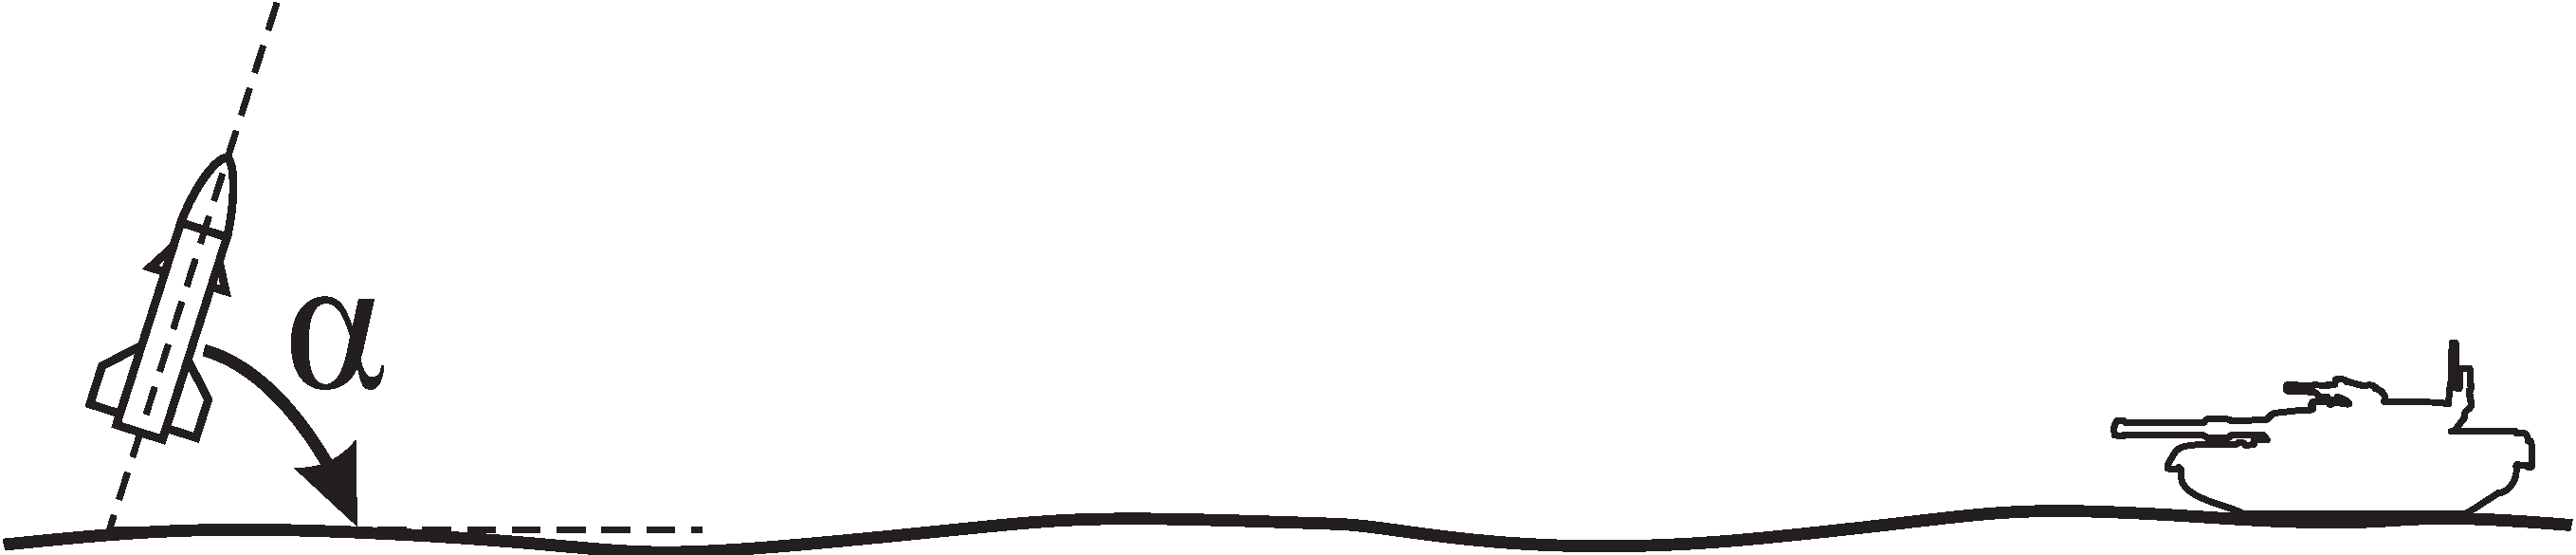
\includegraphics[width=0.475\textwidth]{rys05/alfa1} & 
  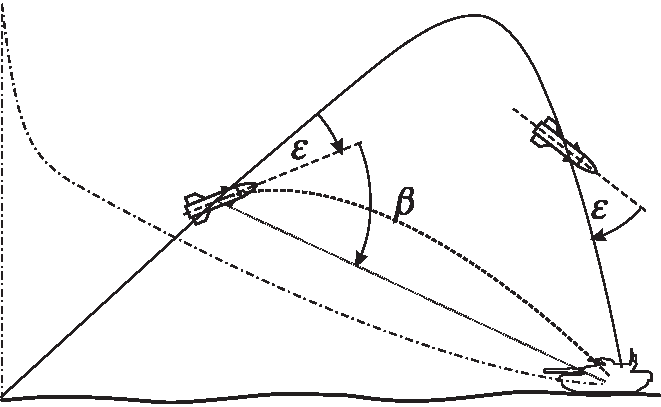
\includegraphics[width=0.475\textwidth]{rys05/beta1}
	% jeli obraki s rnej wysokoci, mona je wyrwna do gry stosujc vtop jak niej
	% \vtop{\vskip-2ex\hbox{{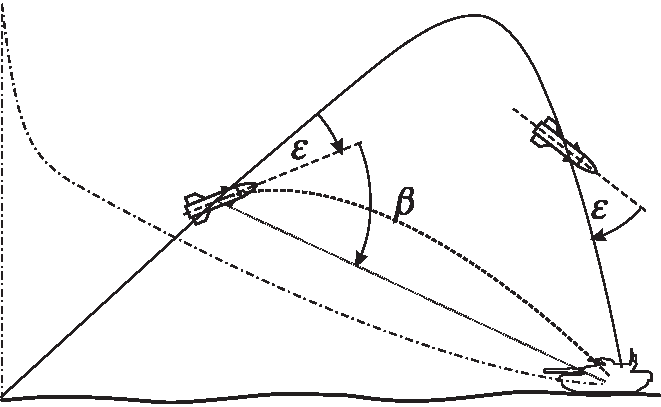
\includegraphics[width=0.475\textwidth]{rys05/beta1}}}} &
	% \vtop{\vskip-2ex\hbox{{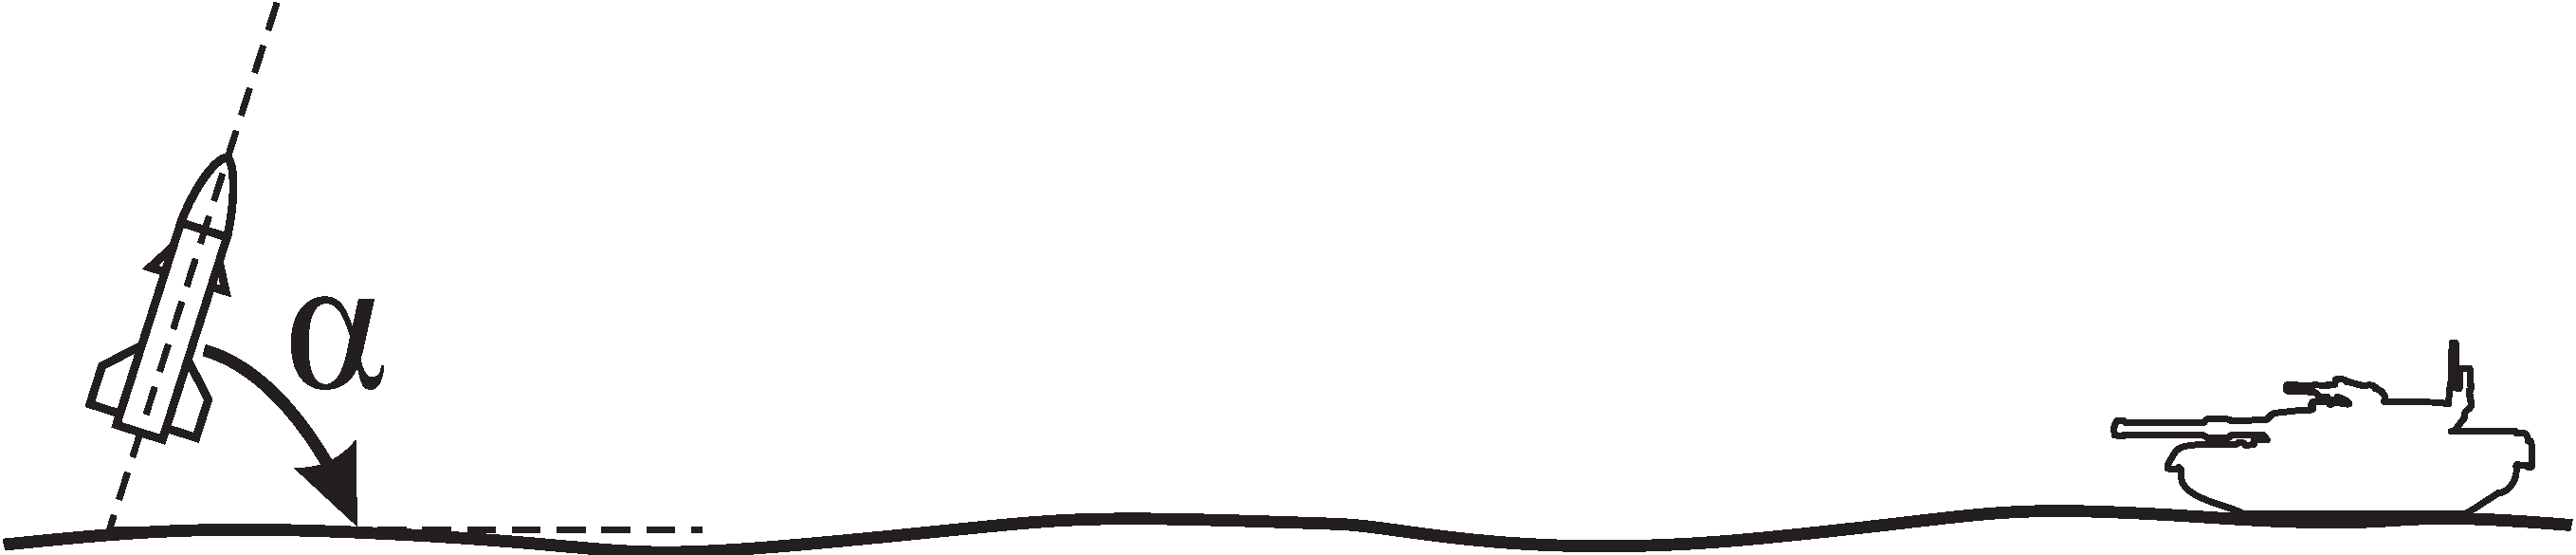
\includegraphics[width=0.475\textwidth]{rys05/alfa1}}}} 
  \end{tabular}
 \caption{Wyznaczanie trajektorii lotu rakiety: 
 a) trzy podejcia, b) podejcie praktyczne}
 \label{fig:alfabeta}
\end{figure}
\end{lstlisting}

\begin{figure}[ht]
	\centering
		
\includegraphics[width=0.3\linewidth]{rys05/kanji-giri}
	\caption{Dwa znaki kanji -- giri}
	\label{fig:kanji-giri}
\end{figure}

\begin{figure}[htb]
  \centering
	\begin{tabular}{@{}ll@{}}
	a) & b) \\
  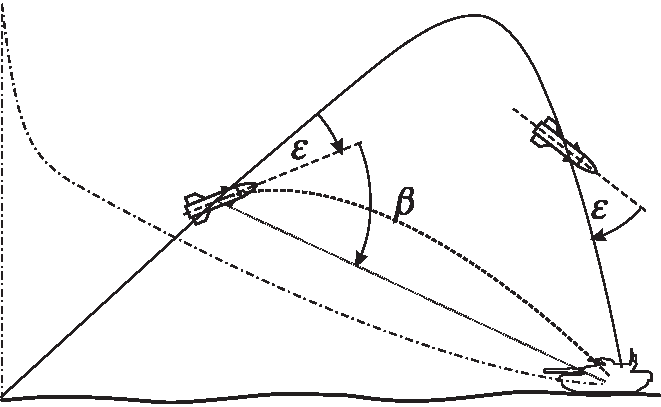
\includegraphics[width=0.475\textwidth]{rys05/beta1} & 
	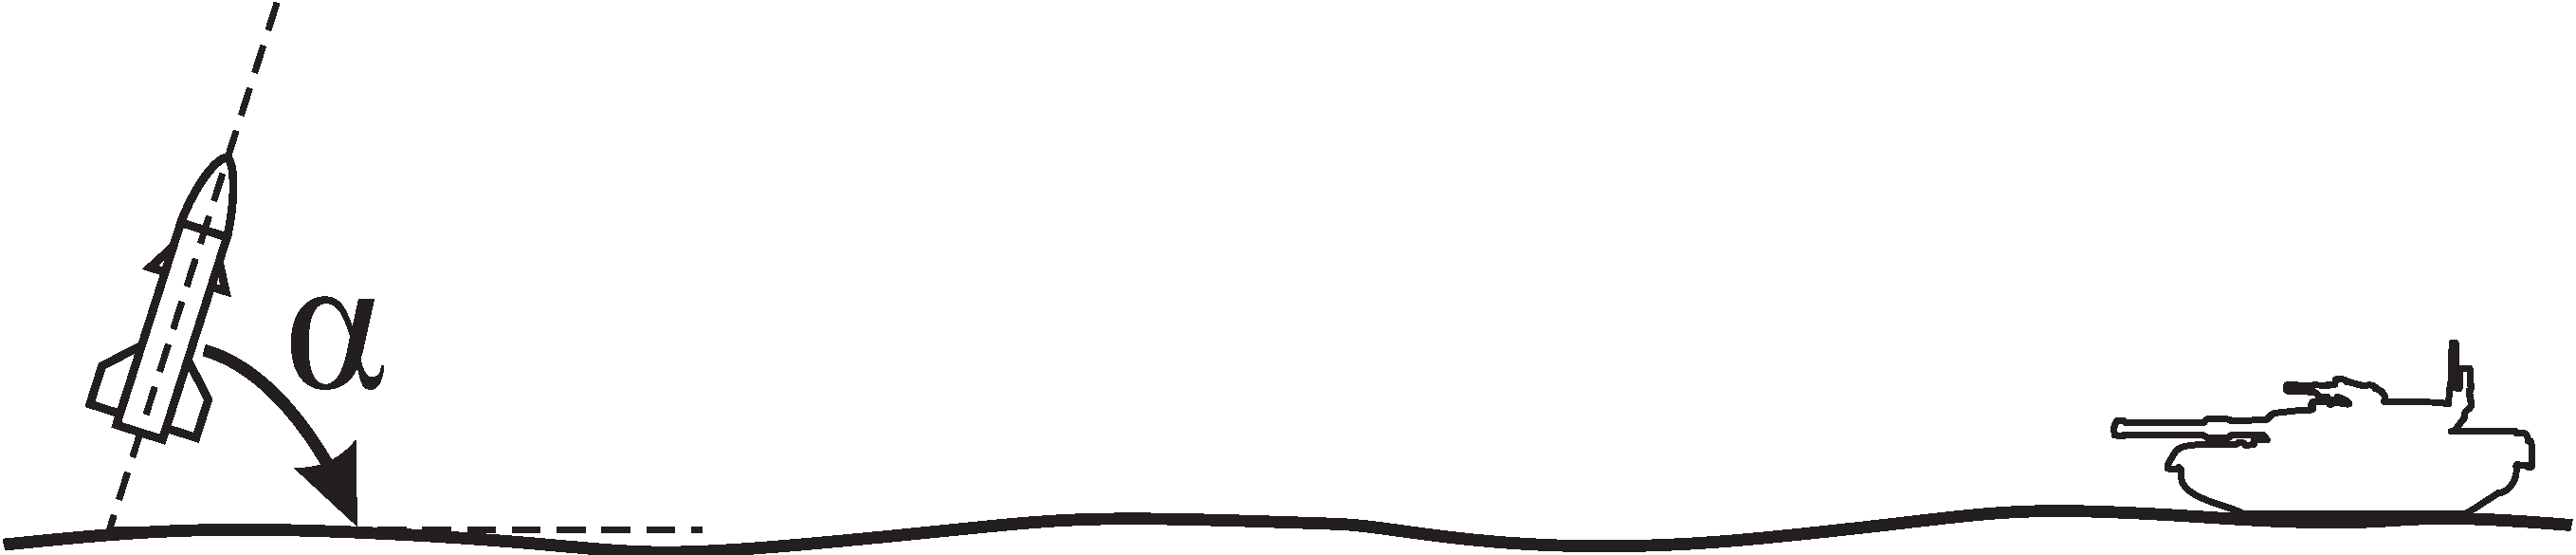
\includegraphics[width=0.475\textwidth]{rys05/alfa1}
	% jeli obraki s rnej wysokoci, mona je wyrwna do gry stosujc vtop jak niej
	% \vtop{\vskip-2ex\hbox{{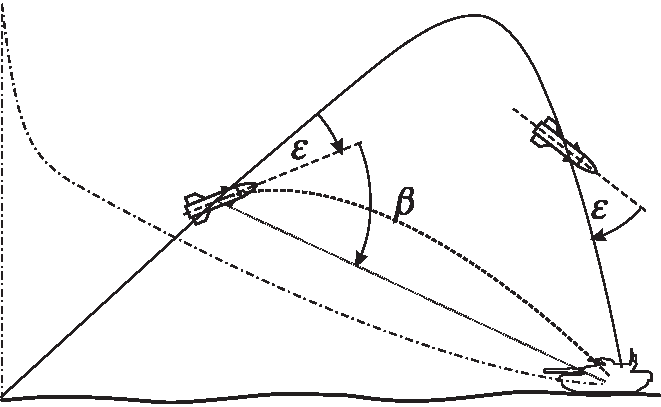
\includegraphics[width=0.475\textwidth]{rys05/beta1}}}} &
	% \vtop{\vskip-2ex\hbox{{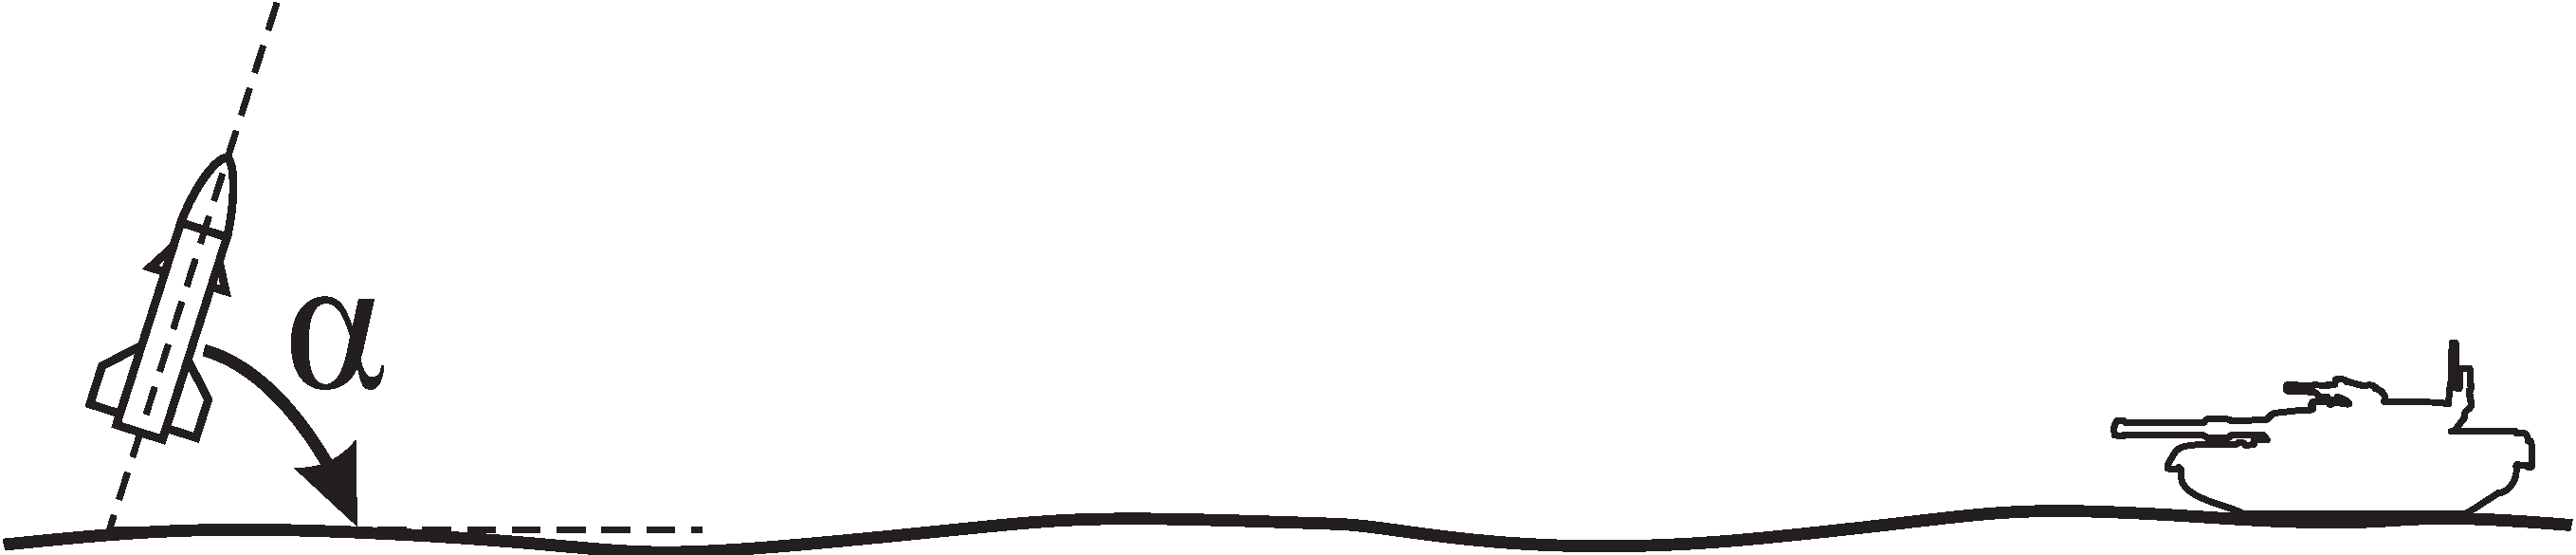
\includegraphics[width=0.475\textwidth]{rys05/alfa1}}}} 
	\end{tabular}
  \caption{Wyznaczanie trajektorii lotu rakiety: a) trzy podejcia, b) podejcie praktyczne}
  \label{fig:alfabeta}
\end{figure}

Grafiki wektorowe powinny by dostarczone w plikach o formacie pdf. Rozmiar strony w~pliku pdf powinien by troszeczk wikszy ni zamieszczona na nim grafika (prosz spojrze na przykady grafik wykorzystanych w niniejszym szablonie). Chodzi o to, aby na rysunku nie pojawiaa si niepotrzebna biaa przestrze. Grafiki rastrowe (gwnie zrzuty z ekranu bd zdjcia) powinny by dostarczane w plikach o formacie png z~kompresj bezstratn. Zastosowanie kompresji stratnej, jak jpg, wprowadza niepotrzebne artefakty. Podobnie jak w przypadku grafik wektorowych, grafiki rastrowe nie powinny mie biaych marginesw.

Na rysunkach nie powinno stosowa si 100\% czarnego wypenienia, bo robi si plamy przebijajce si przez kartk. Zamiast tego wypenienie powinno by ok.\ 90\% czerni.

Czcionka na rysunkach nie moe by wiksza od czcionki wiodcej tekstu (jedyny wyjtek to np.\ jakie nagwki).
Naley stosowa czcionk kroju Arial, Helvetica bd tego samego kroju co czcionka dokumentu (\texttt{texgyre-termes}). 

Jeli na jednym rysunku pojawi si ma kilka grafik, to zamiast stosowa \texttt{subfigure} lub inne otoczenia naley wstawi grafiki w tabel, opisa j indeksami a) i b), a potem odnie si do tego w podpisie (rys.~\ref{fig:alfabeta}).
Czasem pomaga w pozycjonowaniu rysunkw uycie komendy:
\verb+\vtop{\vskip3ex\hbox{\includegraphics[width=0.475\textwidth]{nazwa}}}+

Na rysunkach nie wolno naduywa kolorw oraz ozdobnikw (wiele narzdzi do tworzenia diagramw dostarcza grafik z cieniowaniem, gradacj kolorw itp.\  co niekoniecznie przekada si na czytelno rysunku).

Podczas rozbienia zrzutw z ekranu naley zadba o to, by taki zrzut by czytelny po wydrukowaniu. Czyli aby pojawiajce si literki byy wystarczajco due, a przestrzenie bez treci -- relatywnie mae.
Przystpujc do robienia zrzutu trzeba odpowiednio wyskalowa elementy na ekranie. Na przykad robic zrzut z przegldarki FF najpierw naley wcisn CTR--0 (domylne skalowanie), potem CTR--{}- (zmniejszenie skali o stopie). Potem dobrze jest zawzi okno przegldarki tak, by interesujca tre wypenia je w caoci. Jeli na obserwowanej stronie jest zbyt duo pustych obszarw, to naley je jako zawzi (sterujc wielkoci okna przegldarki lub aktywnymi elementami interfejsu uytkownika). Zrzut bowiem wcale nie musi by odzwierciedleniem 1:1 domylnego ukadu obserwowanych elementw. Wane jest, by na zrzucie z ekranu pokaza interesujcy, opisywany fragment i eby ten fragment by czytelny.
	
Czasem problemem jest tworzenie zrzutw z ekranu, gdy wystpuj na nim dane wraliwe. Istniej dwa sposoby na radzenie sobie z tym problemem.
Pierwszy polega na zastpieniu w~systemie danych danych rzeczywistych danymi testowymi -- wygenerowanymi tylko do celw prezentacji.
Zrzut robi si wtedy na bazie danych testowych.
Drugi polega na wykonaniu zrzutu z~ekranu, na ktrym pokazano dane rzeczywiste, i nastpnie zamianie tych danych ju w pliku graficznym
za pomoc odpowiedniego edytora (np.~\texttt{gimp}). Czyli oryginalny zrzut z ekranu naley otworzy w edytorze, a potem
nadpisa oryginalny tekst wasnym tekstem. Konieczne jest wtedy dobranie odpowiednich czcionek aby nie byo wida
wprowadzonych zmian. 
\begin{quotation}
Uwaga: takie manipulowanie zrzutami jest usprawiedliwione jedynie w przypadku koniecznoci ochrony danych wraliwych czy te lepszego pokazania wybranych elementw. Nie moe to prowadzi generowania faszywych rezultatw!!!
\end{quotation}

\section{Wstawianie kodu rdowego}
Kod rdowy mona wstawia jako blok tekstu pisany czcionk maszynow. Uywa si do tego otoczenie \verb?\lstlisting?. W atrybutach otoczenia mona zdefiniowa tekst podpisu wstawianego wraz z numerem nad blokiem, etykiet do tworzenia odwoa, sposb formatowania i~inne ustawienia. Zaleca si stosowanie w tym otoczeniu nastpujcych parametrw:
\begin{lstlisting}[basicstyle=\footnotesize\ttfamily]
\begin{lstlisting}[label=list:req1,caption=Initial HTTP Request,
                   basicstyle=\footnotesize\ttfamily]
\end{lstlisting}
Szczeglnie przydatne podczas wstawiania wikszej iloci kodu rdowego jest zastosowanie parametru \verb+basicstyle=\footnotesize\ttfamily+. Dziki niemu zmniejsza si czcionka, a~przez to na stronie mona zmieci dusze linijki kodu. Uycie tak zdefiniowanego parametru nie jest jednak sztywnym zaleceniem. Wielko czcionki mona dobiera do potrzeb. 
{\belowcaptionskip=-10pt
\begin{lstlisting}[label=list:req1,caption=Initial HTTP Request,
                   basicstyle=\footnotesize\ttfamily]
GET /script/Articles/Latest.aspx HTTP/1.1
Host: www.codeproject.com
Connection: keep-alive
Cache-Control: max-age=0
Accept: text/html,application/xhtml+xml,application/xml
User-Agent: Mozilla/5.0 ...
Accept-Encoding: gzip,deflate,sdch
Accept-Language: en-US...
Accept-Charset: windows-1251,utf-8...
\end{lstlisting}
}
Mona te sformatowa kod bez stosowania numerowanego podpisu (wtedy nie zamieszcza si \texttt{caption} na licie atrybutw).
\begin{lstlisting}[basicstyle=\footnotesize\ttfamily]
GET /script/Articles/Latest.aspx HTTP/1.1
Host: www.codeproject.com
Connection: keep-alive
Cache-Control: max-age=0
Accept: text/html,application/xhtml+xml,application/xml
User-Agent: Mozilla/5.0 ...
Accept-Encoding: gzip,deflate,sdch
Accept-Language: en-US...
Accept-Charset: windows-1251,utf-8...
\end{lstlisting}

Istnieje moliwo wstawiania kodu rdowego w biecej linijce tekstu. Mona to zrobi na kilka sposobw:
\begin{itemize} 
\item korzystajc z polecenia \verb?\texttt? ustawiajcego czcionk maszynow, jak w przykadzie \texttt{tutaj} (efekt zastosowania komendy \verb?\texttt{tutaj}?). Problemem jednak mog okaza si znaki podkrelenia i inne znaki kontrolne.
\item korzystaj z otoczenia \verb?\verb? zapewniajcego wypisanie kodu czcionk maszynow jak w~przykadzie \verb|tutaj| (efekt zastosowania komendy \verb?\verb|tutaj|?). Problemem jest to, e polecenie \verb?\verb? nie potrafi ama duszego tekstu.
\item korzystajc z polecenia \verb?\lstin? umoliwiajcego wypisanie kodu czcionk ustawian w~opcjach jak w przykadzie
\lstset{basicstyle=\ttfamily}\lstinline{tutaj} (efekt komendy \verb+\lstset{basicstyle=\ttfamily}\lstinline{tutaj}+) lub \lstinline[basicstyle=\ttfamily]=tutaj= (efekt komendy \verb+\lstinline[basicstyle=\ttfamily]=tutaj=+).
\end{itemize}

\section{Wykaz literatury oraz cytowania}
\label{sec:literatura}
Cytowania powinny by zamieszczane w tekcie z uyciem komendy \verb+\cite{}+. Jej argumentem powinien by klucz cytowanej pozycji (lub lista kluczy  rozdzielonych przecinkiem bez spacji, jeli takich pozycji w danym miejscu cytuje si wicej) jaki jest uywany w bazie danych bibliograficznych (plik \texttt{dokumentacja.bib}). Po kompilacji \texttt{bibtex} i \texttt{pdflatex} w tekcie pojawia si waciwy odsyacz do pozycji w wykazie literatury (ujty w kwadratowe nawiasy -- zgodnie z~tym, co definiuje styl \texttt{plabbrv.bst}), za w samym wykazie (rozdzia Literatura) -- zacytowana pozycja. Przykadem cytowania jest: ,,dobrze to opisano w pracach~\cite{JS07,SQL2}'' (gdzie zastosowano komend \verb?\cite{JS07,SQL2}?).

Co do zawartoci rekordw bibliograficznych - style bibtexowe potrafi ,,skraca'' imiona (czyli wstawia, jeli taka wola, inicjay zamiast penych imion). Niemniej dobrze jest od razu przyj jak konwencj. Proponuje si, aby w rekordach od razu wstawiane byy inicjay zamiast penych imion.

Niekiedy tytuy prac zawieraj wyrazy z duymi i maymi literami. Takie tytuy naley bra w podwjne nawiasy klamrowe, aby \texttt{bibtex} nie zamieni ich na posta, w ktrej poza pierwsz liter pozostae s mae.

Jeli jaki cytowany zasb pochodzi z Internetu, to jego rekord w pliku \texttt{bib} powinien wyglda jak niej.
\begin{lstlisting}[basicstyle=\footnotesize\ttfamily]
@INPROCEEDINGS{SQL2, 
  title={{A MySQL-based data archiver: preliminary results}}, 
  author={Bickley, M. and Slominski, Ch.},
  booktitle = {{Proceedings of ICALEPCS07}},
	month = oct,
	day = {15--19},
	year={2007}, 
  note={\url{http://www.osti.gov/scitech/servlets/purl/922267} 
	[dostp dnia 20 czerwca 2015]}
}
\end{lstlisting}
A to inny przykad rekordu danych bibliograficznych:
\begin{lstlisting}[basicstyle=\footnotesize\ttfamily]
@TechReport{JS07,
	author = {Jdrzejczyk, J. and rdka, B.},
	title  ={Segmentacja obrazw metod drzew decyzyjnych},
	year = {2007},
	institution = {Politechnika Wrocawska, Wydzia Elektroniki}
}
\end{lstlisting}

\section{Indeks rzeczowy}
\label{sec:indeks}
Generowanie indeksu \index{generowanie!-- indeksu} po trosze wyglda jak generowanie wykazu literatury \index{generowanie!-- wykazu literatury}-- wymaga kilku krokw. Podczas pierwszej kompilacji \texttt{pdflatex} generowany jest plik z rozszerzeniem \texttt{*.idx} (zawierajcy ,,surowy indeks''). Nastpnie, bazujc na tym pliku, generowany jest plik z rozszerzeniem \texttt{*.ind} zawierajcy sformatowane dane. Ten krok wymaga uruchomienia odpowiedniego narzdzia oraz zastosowania plik z definicj stylu \texttt{Dyplom.ist}. W kroku ostatnim dokonuje si kolejnej kompilacji \texttt{pdflatex} (dziki niej w wynikowym dokumencie pojawi si Indeks rzeczowy). Domylnie Indeks rzeczowy zostanie sformatowany w~ukadzie dwukolumnowym.

Oczywicie aby to wszystko zadziaao w kodzie szablonu naley umieci odpowiednie komendy definiujce elementy indeksu rzeczowego (\verb?\index?) oraz wstawiajce sformatowany Indeks rzeczowy do dokumentu wynikowego (\verb?\printindex?). Wicej informacji o tworzeniu indeksu rzeczowego mona znale na stronie \url{https://en.wikibooks.org/wiki/LaTeX/Indexing}. Poniej przedstawiono przykady komend uytych w szablonie do zdefiniowania elementw indeksu rzeczowego:
\begin{itemize}
\item \verb?\index{linia komend}? -- pozycji gwna.
\item \verb?\index{generowanie!-- indeksu}? -- podpozycja.
\end{itemize}

Generowanie pliku \texttt{*.ind} mona inicjowa na kilka sposobw:
\begin{itemize}
\item poprzez wydanie odpowiedniego polecenia bezporednio w linii komend \index{linia komend}
\begin{lstlisting}[basicstyle=\footnotesize\ttfamily]
makeindex Dyplom.idx -t Dyplom.ilg -o Dyplom.ind -s Dyplom.ist
\end{lstlisting}
\item poprzez odpalenie odpowiedniego narzdzia rodowiska. Na przykad w \texttt{TeXnicCenter} definiuje si tzw. \texttt{output profiles}: 
\begin{lstlisting}[basicstyle=\footnotesize\ttfamily]
makeindex "%tm.idx" -t "%tm.ilg" -o "%tm.ind" -s "%tm.ist"
\end{lstlisting}
a samo generowanie pliku \texttt{*.ind} zapewni wybranie pozycji menu \texttt{Build/Makeindex}.
\item korzystajc z odpowiednio sparametryzowanych pakietw i komend wewntrz kompilowanego dokumentu (czyli od razu przy okazji jego kompilacji).
\begin{lstlisting}[basicstyle=\footnotesize\ttfamily]
\DisemulatePackage{imakeidx}
\usepackage[noautomatic]{imakeidx} 
% jeli chcemy, by indeks by generowany automatycznie programem makeindex:
%\usepackage[makeindex]{imakeidx} 
% a tak pono mona przekaza opcje do programu generujcego indeks:
%\makeindex[options=-s podrecznik -L polish -M lang/polish/utf8] 
%\makeindex[options=-s podrecznik]
\makeindex
\end{lstlisting}

Niestety, \texttt{makeindex} jest narzdziem, ktre umieszcza cz pozycji w grupie \texttt{Symbols}, a~nie w grupach zwizanych z literkami alfabetu. W zwizku z czym indeksowany element zaczynajcy si od polskiej literki trafia do grupy \texttt{Symbols}, jak np.~\verb?\index{wiato}?\index{wiato}. Jeli chce si zamieszcza w indeksie symbole matematyczne, to dobrze jest to robi jak w nastpujcym przykadzie: \verb?\index{$asterisk@$\ast$}? \index{$asterisk@$\ast$} czy te \verb?\index{c@$\mathcal{C}$}?\index{c@$\mathcal{C}$}, tj.~dostarczajc przy okazji klucz do sortowania.
Lepiej w tym wzgldzie radz sobie inne narzdzia, jak \texttt{texindy} lub \texttt{xindy} dostpne pod linuxem. Korzystajc z nich uzyskuje si grupy polskich literek w indeksie rzeczowym (hasa zaczynajce si od polskich literek ju nie trafiaj do grupy Symbols). Przykad polecenia wydanego z linii komend, w ktrym wykorzystano \texttt{texindy} zamieszczono poniej (zakadamy kodowanie plikw w UTF8, mona dla niniejszego szablonu zmieni na cp1250):
\begin{lstlisting}[basicstyle=\footnotesize\ttfamily]
texindy -L polish -M lang/polish/utf8 Dyplom.idx
\end{lstlisting}

To polecenie wygeneruje \texttt{Dyplom.ind} o zawartoci:
\begin{lstlisting}[basicstyle=\footnotesize\ttfamily]
\begin{theindex}
  \providecommand*\lettergroupDefault[1]{}
  \providecommand*\lettergroup[1]{%
      \par\textbf{#1}\par
      \nopagebreak
  }

  \lettergroup{G}
  \item generowanie
    \subitem -- indeksu, 27
    \subitem -- wykazu literatury, 27

  \indexspace

  \lettergroup{L}
  \item linia komend, 27

  \indexspace

  \lettergroup{}
  \item \'Swiat\IeC {\l }o, 28

\end{theindex}
\end{lstlisting}


\end{itemize}


Aby mie wiksz kontrol automatyczne generowanie indeksu zostao w niniejszym szablonie wyczone (indeks trzeba wygenerowa samemu, wydajc polecenie \texttt{makeindex} lub zalecane \texttt{texindy}).

\section{Inne uwagi}
Dobrym sposobem na kontrol bdw wystpujcych podczas kompilacji jest wstawianie linijki \verb?\end{document}? w wybranym miejscu dokumentu. Jest to szczeglnie przydatne w przypadkach, gdy bdy te s trudne do zidentyfikowania (gdy wygenerowane przez kompilator numery linii z bdami nie s tymi, w ktrych bdy wystpuj). Wystarczy wtedy przestawi wspomnian linijk do kolejnych miejsc, a znajduj to miejsce, gdzie wystpuje problem.

Aby osign apostrofy maszynowe (czyli takie zoone z samych kresek) naley uy polecenia \verb?"{}jak tutaj{}"? (podwjny apostrof i podwjny apostrof z na wszelki wypadek umieszczonymi nawiasami klamrowymi, nawiasy s potrzebne z tej racji, i podwjny apostrof przed niektrymi literkami zamienia je na literki z akcentami). W efekcie otrzymamy "{}jak tutaj{}". Jeli natomiast apostrofy maj by drukarskie (czyli zoone z kropek i kresek), to naley uy polecenia \verb?,,jak tutaj''? (dwa pojedyncze przecinki i dwa pojedyncze apostrofy). W efekcie otrzymamy ,,jak tutaj''. Mona te uy znakw apostrofw odpowiednio zakodowanych jak tutaj, tylko e czasem trudno pisze si takie apostrofy w rodowiskach kompilacji projektw latexowych.


Oto sposoby ustawienia odstpw midzy liniami:
\begin{itemize}
\item uywajc komendy \verb+\linespread{...}+ (akceptowalne), przy czym atrybutem tej metody jest wspczynnik zaleny od wielkoci
czcionki.  Dla czcionki wiodcej 12pt odstp ptora linii osignie si komend \verb+\linespread{1.241}+. Dla innych czcionek wiodcych wartoci tego parametru s jak w poniszym zestawieniu.
\begin{lstlisting}[basicstyle=\footnotesize\ttfamily]
10pt 1.25 dla \onehalfspacing 
     1.667 for \doublespacing, 
		 poniewa ,,basic ratio'' = 1.2 
		(\normalfont posiada \baselineskip rozmiaru 12pt)
11pt 1.213 dla \onehalfspacing oraz 1.618 dla \doublespacing, 
     poniewa ,,basic ratio'' = 1.236 
		(\normalfont posiada \baselineskip rozmiaru 13.6pt)
12pt 1.241 dla \onehalfspacing oraz 1.655 dla \doublespacing, 
     poniewasince ''basic ratio'' is 1.208 
		(\normalfont has a \baselineskip of 14.5pt)
\end{lstlisting}
Kopot w tym, e raz ustawiony odstp bdzie obowizywa do wszystkich czcionek (nie dziaa tu adem mechanizm zmiany wspczynnika w zalenoci od wielkoci czcionki akapitu).

\item uywajc pakietu \texttt{setspace} (niezalecane). Poniewa klasa \texttt{memoir} emuluje pakiet \texttt{setspace}, w preambule dokumentu naleaoby umieci:
\begin{lstlisting}[basicstyle=\footnotesize\ttfamily]
\DisemulatePackage{setspace}
\usepackage{setspace}
\end{lstlisting}
a potem mona ju sterowa odstp komendami:
\begin{lstlisting}[basicstyle=\footnotesize\ttfamily]
\singlespacing
\onehalfspacing
\doubelspacing
\end{lstlisting}
Ten sposb pozwala na korzystanie z mechanizmu automatycznej zmiany odlegoci linii w~zalenoci od wielkoci czcionki danego akapitu.
\item korzystajc bezporednio z komend dostarczonych w klasie \texttt{memoir} (zalecane):
\begin{lstlisting}[basicstyle=\footnotesize\ttfamily]
\SingleSpacing
\OnehalfSpacing
\DoubleSpacing
\end{lstlisting}
Ten sposb rwnie pozwala na korzystanie z mechanizmu automatycznej zmiany odlegoci linii w zalenoci od wielkoci czcionki danego akapitu.
\end{itemize}

Na koniec jeszcze uwaga o rozmiarze pliku wynikowego. Ot \texttt{pdflatex} generuje pliki \texttt{pdf}, ktre zazwyczaj mogyby by nieco lepiej
skompresowane. Do lepszego skompresowania tych plikw mona uy programu \texttt{ghostscript}. Wystarczy w tym celu wyda komend (pod windowsami):
\begin{lstlisting}[basicstyle=\footnotesize\ttfamily]
gswin64 -sDEVICE=pdfwrite -dCompatibilityLevel=1.4 -dNOPAUSE -dQUIET \
-dSAFER -dBATCH -sOutputFile=Dyplom-compressed.pdf Dyplom.pdf
\end{lstlisting}
W poleceniu tym mona rwnie wstawi opcj \texttt{-dPDFSETTINGS=/prepress} (zapewniajc uzyskanie wysokiej jakoci, zachowanie kolorw, uzyskanie obrazkw w rozdzielczoci 300 dpi). Ze wzgldw licencyjnych ghostscript uywa domylnie algorytmw z kompresj stratn. Przy kompresji moe wic doj do utraty jakoci bitmap.
